\Figref{grafico-resultados} compares the simulation and experimental results
obtained for the same reference signal. Using the \gls{rmse} metric from
\Eqref{rmse} to evaluate the tracking error of the relative temperature
measured by sensor 2.

The simulated system achieved an $\mathrm{RMSE} = 1.3567,^\circ\mathrm{C}$,
while the experimental test resulted in an
$\mathrm{RMSE} = 2.2956,^\circ\mathrm{C}$. In both cases, the combined \gls{pd}
and \gls{ff} control strategy was able to track the reference signal during both
the ramp transient and steady-state regimes at $40\,^\circ\mathrm{C}$,
recovering from the disturbance introduced at the 10-minute mark.

The approximately $0.94,^\circ\mathrm{C}$ increase in the experimental
\gls{rmse} compared with the simulated result indicates good agreement between
the model and the physical system, although the experimental performance was
slightly worse than that predicted by simulation.

\begin{figure}[H]
\centering
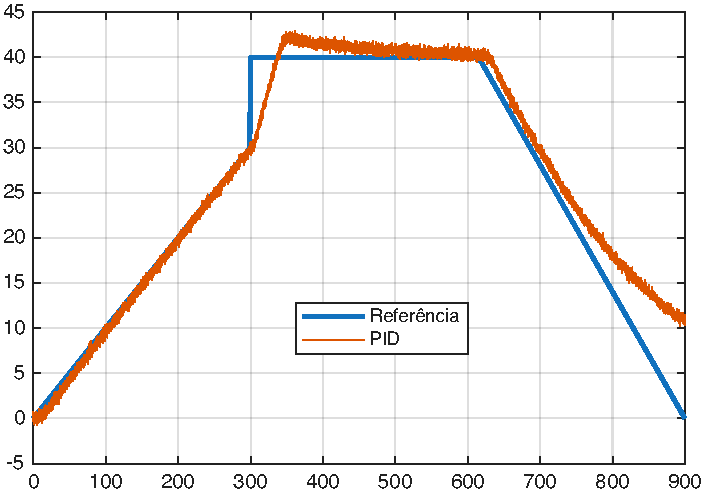
\includegraphics[width=0.9\linewidth]{images/Resultados.pdf}
\caption{Comparison between the simulated and experimental results for tracking
the relative temperature reference measured by sensor 2.}
\figlabel{grafico-resultados}
\end{figure}
